\chapter{Image-Based Disease and Pest Detection}

The detection of plant diseases and pests is a critical task in agriculture, as
early identification can prevent widespread crop damage and reduce yield
losses. Traditional methods of disease detection rely on visual inspection by
human experts, which can be time-consuming and subjective. In recent years, the
application of deep learning techniques, particularly convolutional neural
networks (CNNs), has shown promising results in automating the detection of
plant diseases from images. This chapter explores the use of CNNs for
image-based disease and pest detection in crops, focusing on the dataset, model
architecture, training process, and performance evaluation.\cite{10.3389/fpls.2016.01419}

\begin{figure}[h!]
    \centering
    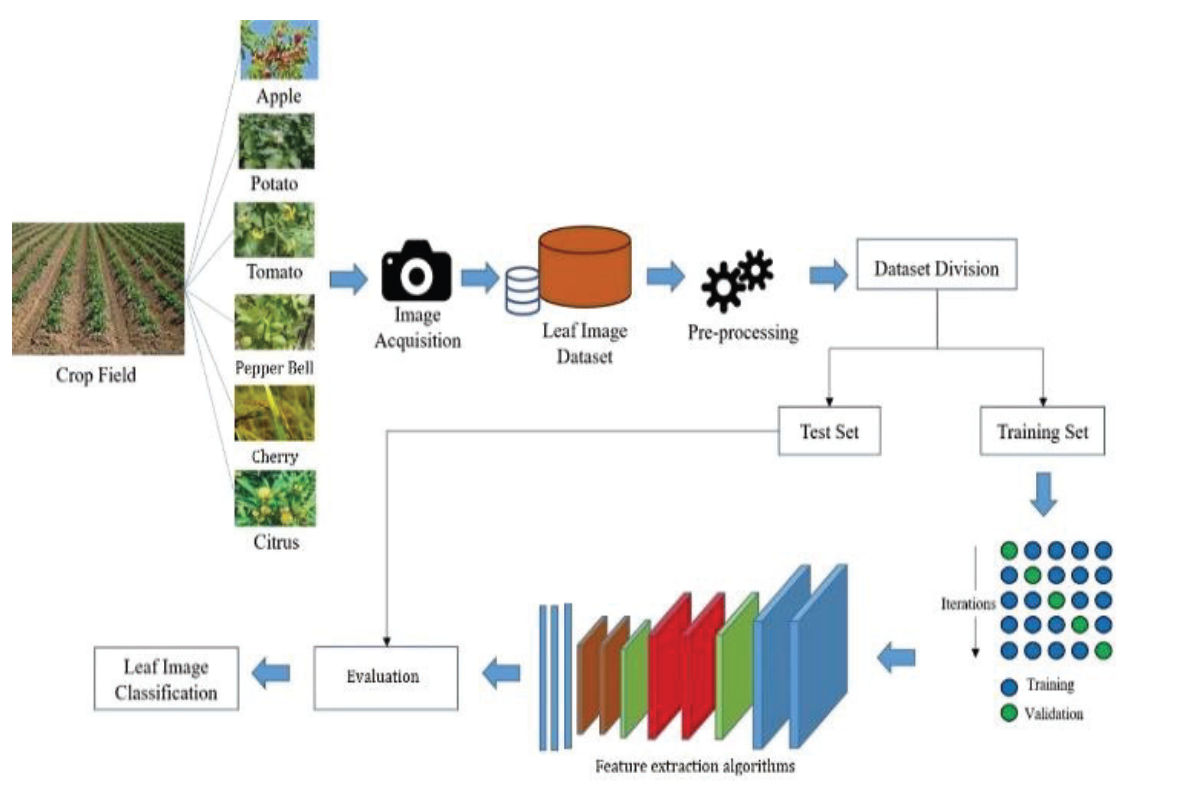
\includegraphics[width=0.8\textwidth]{cnn_architecture_diagram.png}
    \caption{Convolutional Neural Network (CNN) Architecture for Disease Detection.}
    \label{fig:cnn_architecture}
\end{figure}

\section{Dataset}
The model is trained on the PlantVillage dataset, which contains 54,306 images
of plant leaves categorized into 38 classes, representing both healthy and
diseased leaves across various crops. The images are resized to 256x256 pixels
for input into the CNN model. \cite{J2019}

\subsection{Preprocessing}
Before feeding the images into the model, they are preprocessed to enhance the
training efficiency. Preprocessing steps include resizing, normalization, and
data augmentation techniques such as rotation, zoom, and flipping to improve
the model's robustness. \cite{yim2021plantdiseasedetection}

\section{Model Architecture}
The proposed method employs a CNN architecture, which consists of multiple
convolutional layers, max-pooling layers, and fully connected layers. The
architecture extracts features from the input images and classifies them into
healthy or diseased categories.

\subsection{Convolutional Layers}
Convolutional layers are the foundation of CNNs. Each convolutional layer
applies filters to the input images to detect specific features, such as edges,
textures, and patterns. \cite{oshea2015introductionconvolutionalneuralnetworks}

\subsection{Pooling Layers}
Pooling layers perform down-sampling operations to reduce the spatial
dimensions of the feature maps. Max pooling is the most commonly used
technique, where the maximum value within a sliding window is selected.

\subsection{Fully Connected Layers}
After feature extraction, fully connected layers map the features to output
classes representing different plant diseases.

\section{Training and Evaluation}
The CNN model is trained using the PlantVillage dataset with 80\% of the data
used for training and 20\% for testing. The model is optimized using the Adam
optimizer, and the categorical cross-entropy loss function is employed. The
training process is carried out for ten epochs.

\subsection{Performance Metrics}
The model's performance is evaluated using accuracy and loss metrics. The
trained model achieves an accuracy of 95\% on the training data and 94\% on the
test data, demonstrating its effectiveness in classifying plant diseases.

\section{Fine-tuning the Model}
Fine-tuning is an essential step in improving the model's accuracy by
leveraging pre-trained models. Below is an example of fine-tuning a pre-trained
CNN model (e.g., VGG16) on the PlantVillage dataset. \cite{radenović2018finetuningcnnimageretrieval}

\begin{lstlisting}[language=Python, caption=Fine-tuning a Pre-trained CNN]
from tensorflow.keras.applications import VGG16
from tensorflow.keras.preprocessing.image import ImageDataGenerator
from tensorflow.keras.layers import Dense, Flatten
from tensorflow.keras.models import Model
from tensorflow.keras.optimizers import Adam

# Load the pre-trained VGG16 model
base_model = VGG16(weights='imagenet', include_top=False, input_shape=(256, 256, 3))

# Freeze the layers of the pre-trained model
for layer in base_model.layers:
    layer.trainable = False

# Add custom layers on top of the base model
x = Flatten()(base_model.output)
x = Dense(128, activation='relu')(x)
x = Dense(64, activation='relu')(x)
predictions = Dense(38, activation='softmax')(x)

# Define the final model
model = Model(inputs=base_model.input, outputs=predictions)

# Compile the model
model.compile(optimizer=Adam(learning_rate=0.0001), loss='categorical_crossentropy', metrics=['accuracy'])

# Data augmentation
train_datagen = ImageDataGenerator(rescale=1./255, rotation_range=20, width_shift_range=0.2, height_shift_range=0.2, horizontal_flip=True)
test_datagen = ImageDataGenerator(rescale=1./255)

# Load training and testing data
train_generator = train_datagen.flow_from_directory('data/train', target_size=(256, 256), batch_size=32, class_mode='categorical')
test_generator = test_datagen.flow_from_directory('data/test', target_size=(256, 256), batch_size=32, class_mode='categorical')

# Train the model
history = model.fit(train_generator, epochs=10, validation_data=test_generator)

# Evaluate the model
loss, accuracy = model.evaluate(test_generator)
print(f'Test Accuracy: {accuracy * 100:.2f}%')
\end{lstlisting}